\documentclass[11pt]{article}

\title{MWF toolbox for EEG artifact removal - Manual}
\author{Ben Somers, Tom Francart, Alexander Bertrand}
\date{November 2017}

\usepackage{a4wide}
\usepackage{enumitem}
\usepackage[hidelinks]{hyperref}
\usepackage{listings}
\usepackage{graphicx}

\hypersetup{
    colorlinks=true,
    linkcolor=black,
    filecolor=black,      
    urlcolor=blue,
    citecolor=black,
}
\urlstyle{same}

\begin{document}

\maketitle
\tableofcontents
\pagebreak

\section{Introduction}

This document is the user manual for the MATLAB toolbox for EEG artifact removal based on the Multi-channel Wiener Filter~(MWF). The MWF algorithm for EEG artifact removal is described and validated in detail in~\cite{somers2018generic}.

The toolbox is available online at \url{www.github.com/exporl/mwf-artifact-removal}. This manual is written for the 1.0 release version. New features may be added later.

\section{Repository contents}

The GitHub repository contains the following folders and files:

\begin{itemize}[noitemsep]
\item[-] \textbf{mwf folder}: contains all required MATLAB code for using the MWF.
\item[-] \textbf{doc folder}: contains manual and demo files.
\item[-] \textbf{paper folder}: contains code for generating the results and figures described in the paper~\cite{somers2018generic}. These are only included for reproducibility of the paper, they are not needed for your own use of the MWF.
\item[-] \textbf{.gitignore}, \textbf{README} and \textbf{LICENSE} files. Note that the licence (\href{www.github.com/exporl/mwf-artifact-removal/blob/master/LICENSE.md}{online link}) under which this code is distributed does not allow usage for commercial purposes.
\end{itemize}

\newpage
\section{Quick start guide}
\label{sec:quickstart}

All functions needed to perform MWF-based EEG artifact removal are in the mwf folder. Before starting, make sure that this folder is added to the MATLAB path.

The MWF first requires examples of EEG with and EEG without artifacts. Based on this segmentation of the EEG data, the MWF can be computed and applied in order to remove the artifacts. This two-step approach is fully implemented in the toolbox.
\\

\textbf{Step 1: EEG segmentation.} In the toolbox, this step is performed by manual marking of the data using a GUI\footnote{The GUI makes use of EEGLAB functionality. In order to visualize the EEG for manual marking, it is required to download the EEGLAB MATLAB toolbox \url{www.sccn.ucsd.edu/eeglab/index.php}. Make sure the EEGLAB toolbox is added to the MATLAB path as well.}. If you have your EEG data matrix in the the MATLAB workspace (channels x samples), you can obtain the artifact mask by calling

\begin{lstlisting}[frame=single, language=matlab]
    mask = mwf_getmask(EEG, samplerate)
\end{lstlisting}

This pops up the GUI in which artifacts can be marked by clicking and dragging over them. When done, clicking the 'Save Marks' button will close the GUI and the function returns a binary (1 x samples) mask. In this mask, ones correspond to artifact segments, and zeros correspond to clean data. Optionally, the mask may contain NaNs which indicate segments to be ignored from the MWF computation (i.e. they belong neither to the artifact nor the clean segments). Section~\ref{tips} contains extra tips on annotating artifacts.
\\

\textbf{Important note:} all segments that are not marked and come BEFORE the lasted marked segment will be treated as artifact-free samples in the training of the filter. The samples that come after the last marked segment are not used in the filter design. In other words: the filter design assumes that ALL artifacts before the last marked artifact are marked.

Because samples after the lasted marked segment are ignored, it is not necessary to go through the entire signal to mark all the artifacts. It is sufficient to annotate only the first few seconds or minutes of the signal. However, the more artifacts are marked, the better the filter design will be.

It is not required to manually mark the entire signal in the GUI; it suffices to go through the first few seconds or minutes of data and mark all artifacts you see there. All samples after the last marked artifact segment are set to NaN, which will exclude them from the data used to train the MWF. However, there are two important considerations:
\begin{itemize}[noitemsep]
\item[-] The more artifacts are marked, the better the filter designed to remove those artifacts will be.
\item[-] In addition to the previous point, there should be enough clean (unmarked) segments before the last marked artifact for a good filter design.
\end{itemize}

The artifact detection step is not inherently a part of the MWF algorithm: if you prefer, you can also use a different method for acquiring the artifact mask (e.g. an automatic method, for example based on thresholding,\ldots). The mask needs to consist of ones and zeros, and have the same length as the EEG data.
\\

\textbf{Step 2: MWF artifact removal} is performed by calling the mwf\_process function. It requires the EEG data, the mask indicating which segments are artifacts, and optionally a delay parameter:

\begin{lstlisting}[frame=single, language=matlab]
    clean_EEG = mwf_process(EEG, mask, delay)
\end{lstlisting}

This will return the artifact-free EEG in the clean\_EEG variable. Using the optional delay parameter includes temporal information into the filter, leading to better artifact removal but may increase processing time. If omitted, the default value is zero. See~\cite{somers2018generic} for more details.

\section{Function documentation}

The MATLAB m-files of the MWF functions contain detailed documentation about the functions usage, inputs/outputs, and some examples. In addition, the mwf\_demo.m file in the doc folder contains a step-by-step demonstration of MWF usage on artifact removal in some example EEG data. For basic use, the in-file documentation, the demo, and the quick start guide in section~\ref{sec:quickstart} should suffice. The following subsections contain additional documentation on some advanced usage of the MWF functions.

\subsection{mwf\_getmask}

\begin{lstlisting}[frame=single, language=matlab]
[mask] = mwf_getmask(EEG, Fs, cacheID, cachepath, redo, mode)
\end{lstlisting}

\subsubsection{Input arguments}

The mwf\_getmask function implements the artifact selection GUI based on EEGLAB's plotting functionality. For basic usage, it is sufficient to provide the \textbf{EEG} data (channels x samples) and the EEG sample rate \textbf{Fs}. The other arguments are related to caching (i.e. saving) the created mask for later reuse:

\begin{itemize}[noitemsep]
\item[-] \textbf{cacheID} is a character string which will allow identification of a cached mask, e.g. ``subject1\_trial2''. The mask will be saved in a matfile with the cacheID in the name, in the folder specified by cachepath (see next point). If no cacheID is given, the mask will not be saved.
\item[-] \textbf{cachepath} is a string specifying the path where to save the cache. It is recommended to create a dedicated cache folder and store all cached masks in there. If unspecified, the current directory will be used.
\item[-] \textbf{redo}. Normally, if you specify a cacheID and cachepath, the function will retrieve a saved mask if it exists. Setting the redo flag to true will allow you to redo the artifact marking regardless of whether there exists a cache already. The existing cache entry matching the cacheID and cachepath will be overwritten. By default, redo is false.
\end{itemize}

Caching is very handy as it allows you to easily re-run the analysis without having to mark the artifacts again. For example usage of the caching, see the documentation in mwf\_getmask.m.

The last argument \textbf{mode} specifies the GUI to use. By default, EEGLAB is used (mode~0). It is possible to use the EyeBallGUI\footnote{This MATLAB toolbox can be found at \url{http://eyeballgui.sourceforge.net}} (mode~1), a different MATLAB toolbox, but its usage is no longer supported by the MWF toolbox and therefore not recommended.

\subsubsection{Output}

The \textbf{mask} variable contains the user's markings in a vector of the same length as the input EEG data. At time points where an artifact was marked, the vector contains ones, at unmarked time points the mask vector contains zeros. All samples after the last marked artifact segment are set to NaN, which will exclude them from the data used to train the MWF. This allows the user to only mark the first part of the signals instead of having to mark everything.

\subsubsection{Using the GUI for artifact marking}

Running this function will pop up an EEGLAB plot as depicted in figure~\ref{fig:getmask}. The EEG display can be customized (e.g. number of channels in view, time range to show, scale,\ldots). The user can scroll through channels and time points to inspect the EEG for undesired artifacts. Artifacts can be marked by click-and-dragging over segments, which will highlight the segments as shown in the figure. When finished marking, clicking the ``SAVE MARKS'' button will close the window and build the mask.

\begin{figure}[h]
    \centering
    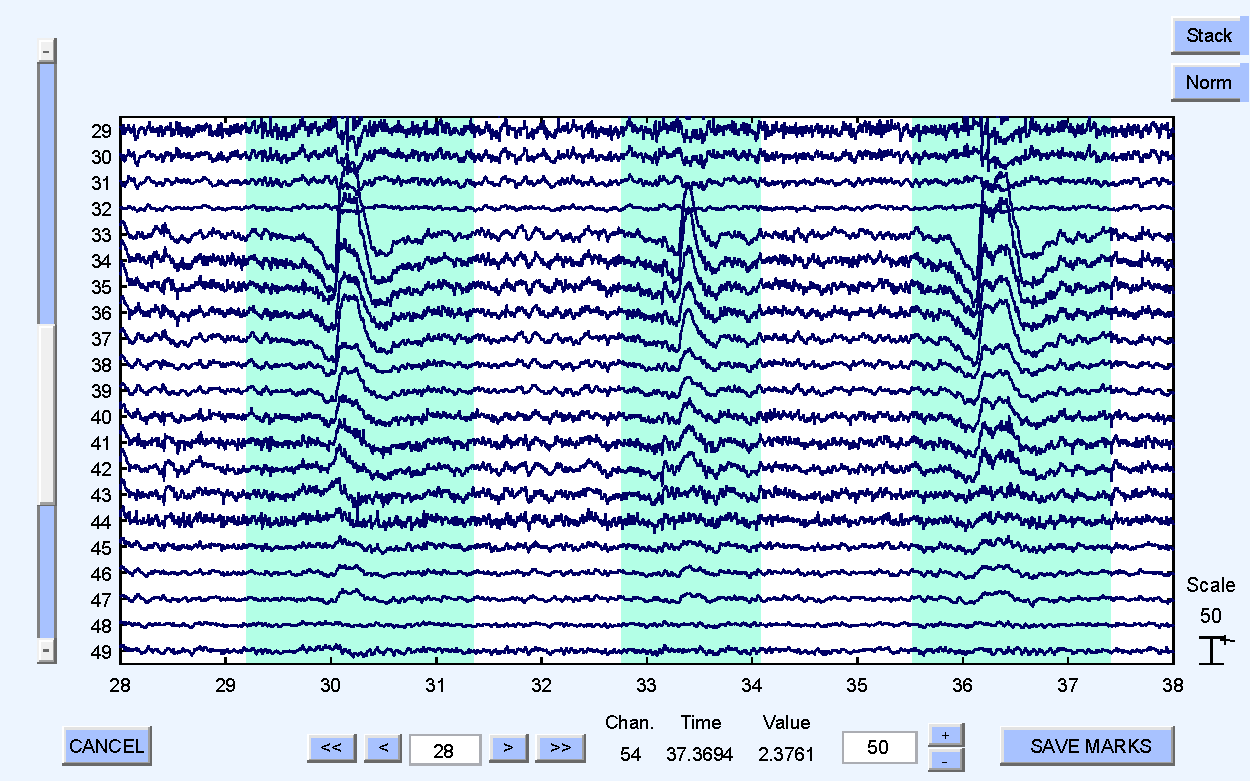
\includegraphics[width=.9\textwidth]{fig_getmask.pdf}
    \caption{Example of marking some eye blink artifacts in the GUI.}
    \label{fig:getmask}
\end{figure}

\subsubsection{Notes}
\label{tips}

\begin{itemize}[noitemsep]
\item[-] All segments that are not marked and come BEFORE the lasted marked segment will be treated as artifact-free samples in the training of the filter. The samples that come after the last marked segment are not used in the filter design. In other words: the filter design assumes that ALL artifacts before the last marked artifact are marked.
\item[-] The more examples of artifacts are marked, the better the MWF design will be.
\item[-] In addition to marking enough examples of artifacts, it is also important to have enough segments of clean (unmarked) EEG data in between the marked artifact  segments.
\item[-] MWF performance decreases quickly if artifacts are ``missed'' and are included in the clean data. However, it is no problem when clean data is included in the artifact markings. Therefore, when marking artifact segments, it is recommended to draw broad windows around the artifacts. If you are unsure whether a segment is artifact or not, it is better to mark it anyway.
\item[-] If you alter the mask after obtaining it with this function, any value other than 1 and 0 will be ignored for the computation of the MWF. You can use this to exclude EEG segments from the training of the MWF (e.g. by setting them to NaN).
\end{itemize}
\vspace{10mm}

\subsection{mwf\_process}

\begin{lstlisting}[frame=single, language=matlab]
[n, d, W, SER, ARR, p] = mwf_process(EEG, mask, delay)
\end{lstlisting}

The mwf\_process function processes the input \textbf{EEG} with the MWF to remove the artifacts as marked in the input \textbf{mask}. An option \textbf{delay} input argument can be specified to include temporal information in the MWF, which will improve artifact removal but increase computation time. The delay should be a positive scalar (samples) and is 0 by default. All other MWF parameters are set to their default values which should work well in general.

The function returns the clean, artifact-free EEG data \textbf{n} and the artifact estimate \textbf{d}. Other outputs are the filter matrix \textbf{W}, the performance measures \textbf{SER} and \textbf{ARR}, and the struct \textbf{p} containing the parameters used for the processing.

The mwf\_process function is a high-level, user-friendly function and should generally yield good results for a well-chosen mask. If the user wants more control over the filter parameters, the functions in the next few subsections can be used.

\newpage
\subsection{mwf\_params}
\label{mwfparams}

\begin{lstlisting}[frame=single, language=matlab]
p = mwf_params(`parameter1', `value1', `parameter2', `value2', ...)
\end{lstlisting}

\subsubsection{Specification of MWF parameters}

This function creates a MATLAB structure \textbf{p} containing key-value pairs of parameters defining the MWF processing. The struct should be passed on to the mwf\_compute function (see section~\ref{mwfcompute}). Parameters can be set by providing their keyword followed by the desired value as an input, for example:
%
\begin{lstlisting}[frame=single, language=matlab]
p = mwf_params(`delay', 5, `rank', `poseig')
\end{lstlisting}
%
Unspecified parameters will be kept at their default value.

The following parameters are able to be set:

\begin{itemize}
\item \textbf{delay}: expects a non-negative integer. Specifies the amount of channel lags, expressed in samples, to incorporate in the filter, e.g. if delay is 5, then all delays from -5,~\ldots,~5 will be included. The default value is 0 (i.e. no delays will be inlcuded).

\item \textbf{rank}: expects one of the following strings (see \cite{somers2018generic} for more details):
\begin{itemize}
\item[-] `full': creates MWF filter where all eigenvalues are retained
\item[-] `poseig': creates MWF filter where only positive eigenvalues are retained (default)
\item[-] `first': creates MWF where only the X largest eigenvalues are retained
\item[-] `pct': creates MWF where only X\% of largest eigenvalues are retained
\end{itemize}

\item \textbf{rankopt}: specify X if `first' or `pct' were selected for the rank parameter. Expects a positive integer (`first') or a percentage (`pct').

\item \textbf{mu}: noiseweighting factor. By default, mu is 1, which results in a regular MWF. If mu $> 1$, a so-called Distortion Weighted MWF (DW-MWF)~\cite{serizel2010integrated} is computed, which allows better artifact estimation, but introduces more noise in the artifact-free segments (i.e. higher ARR but lower SER). The opposite trade-off is true when mu $< 1$ (but greater than 0).

\end{itemize}

\subsubsection{Notes}

\begin{itemize}[noitemsep]
\item[-] In \cite{somers2018generic}, it was shown that there is a benefit of including some delays (e.g. 5 samples) in the MWF design. However, there is a trade-off with computation time.
\item[-] In \cite{somers2018generic}, it was shown that the poseig option for rank generally selects the optimal rank for the MWF, which is why it is the default option.
\item[-] The factor mu allows to trade off artifact estimation quality for clean EEG distortion. It is recommended to leave it at the default value of 1.
\end{itemize}

\newpage
\subsection{mwf\_compute}
\label{mwfcompute}

\begin{lstlisting}[frame=single, language=matlab]
[W, Lambda] = mwf_compute(EEG, mask, p)
\end{lstlisting}

This function computes the MWF based on the input \textbf{EEG}. The EEG is split into artifacted and clean segments using the \textbf{mask}. Any samples corresponding to NaNs in the mask are ignored from the MWF computation. Additional parameters involved in the processing are set in the parameter struct \textbf{p}.

The function returns the MWF matrix \textbf{W}, as well as an ordered diagonal matrix containing the generalized eigenvalues in \textbf{Lambda}. The sizes of W and Lambda will be M~x~M, where M is the number of channels \emph{including delayed channels}. 

\subsection{mwf\_apply}

\begin{lstlisting}[frame=single, language=matlab]
[n, d] = mwf_apply(EEG, W)
\end{lstlisting}

This function applies a precomputed MWF matrix \textbf{W} to the input \textbf{EEG} data. The filtered, artifact-free EEG data \textbf{n} is returned, as well as the estimate of the artifacts \textbf{d}. It may be informative to inspect the pure artifact signal~d to see what the artifacts look like without the rest of the EEG.

Because the compute and apply functionality if split in two different functions, it is possible to compute an MWF on one set of EEG signals with mwf\_compute, and apply it to a different set of EEG signals with mwf\_apply. One restriction is that the number of channels in both EEG sets need to be the same, otherwise the precomputed filter W is incompatible with the EEG test set.

\subsection{mwf\_performance}

\begin{lstlisting}[frame=single, language=matlab]
[SER, ARR] = mwf_performance(EEG, d, mask, d_real)
\end{lstlisting}

This function computes two performance measures SER and ARR, which are defined in \cite{somers2018generic}. The \textbf{SER} is a measure for distortion of clean EEG caused by the filter. The \textbf{ARR} is a measure for artifact estimation accuracy by the filter. Good performance is indicated by both high SER and high ARR. Both values are expressed on a decibel scale.

In order to compute these measures, the function requires the \textbf{EEG} data, as well as the artifact signal \textbf{d} estimated by the MWF, and the \textbf{mask} used to split EEG in artifact and clean segments (NaNs in the mask are ignored). An optional fourth input \textbf{d\_real} can be provided, which should contain the real, ground-truth artifact signal that is estimated by \textbf{d}. Of course, this is only possible to provide for synthetic or simulated EEG data. If d\_real is provided, a more accurate ARR can be computed.

\newpage
\section{Closing remarks}

The MWF-EEG code is distributed freely online in the hope that it may provide a useful method for other researchers in dealing with artifacts in their EEG data. See the \href{www.github.com/exporl/mwf-artifact-removal/blob/master/LICENSE.md}{license file} distributed along with the toolbox for license rights and limitations. If this toolbox is useful for your data analysis, please cite~ \cite{somers2018generic} in any publications that may follow from it.


We are open to any suggestions for interesting features or ways to further improve the toolbox. Communication regarding the MWF-EEG toolbox can be addressed through the GitHub website or directly to \href{mailto:ben.somers@med.kuleuven.be}{ben.somers@med.kuleuven.be}

\begin{thebibliography}{9}

\bibitem{somers2018generic}
  B. Somers, Ben, T. Francart and A. Bertrand,
  ``A generic EEG artifact removal algorithm based on the multi-channel Wiener filter", 
  \textit{Journal of Neural Engineering},
  (2018).
  
\bibitem{serizel2010integrated}
  R. Serizel, M. Moonen, J. Wouters and S.H. Jensen,
  ``Integrated active noise control and noise reduction in hearing aids", 
  \textit{IEEE Transactions on Audio, Speech, and Language Processing},
  18.6 (2018):1137-1146.

\end{thebibliography}

\end{document}